\section{A methodology for the study of feedback-loop systems in Edge Computing}\label{summary:methodology}

\begin{figure}
    \centering
    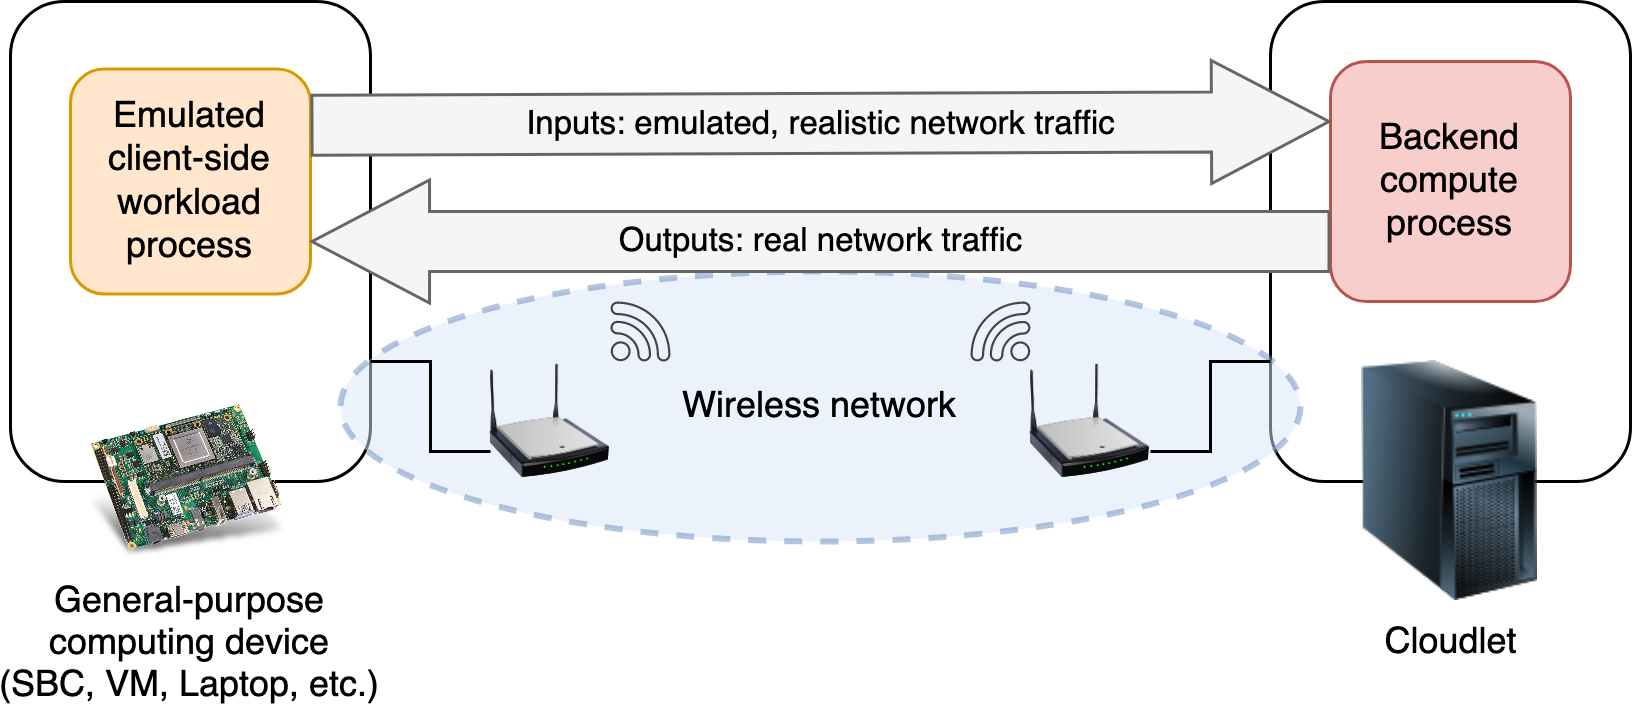
\includegraphics[width=.8\textwidth]{Figs/methodology.png}
    \caption{%
        Overview of the proposed methodology for the study of feedback-loop systems on edge computing infrastructure.
        The  client side of the system is replaced with an emulation executed on a general-purpose computing device.
        The backend/server side of the system along with the network remain unchanged.
    }\label{fig:methodology}
\end{figure}

As discussed above, benchmarking infrastructures for edge-bound applications featuring feedback-loops is challenging, in particular when dealing with applications with high sensitivity to latency (such as \gls{NCS}) or with human involvement (such as \gls{WCA}).
In the following, we introduce our methodological framework for tackling this challenge.

A general overview of our methodology is illustrated in \cref{fig:methodology}.
It is based on the core idea of executing an emulation of the target workload on top of the real hardware on which it is to be deployed.
We replace the client side of the system with a realistic emulation of the desired behaviors; this emulation is implemented in software deployed on \gls{COTS} general-purpose computing devices.
The backend side and the network are not changed.

Two main arguments drive this approach.
One, the difficulty of scaling the number of clients in these systems in a research context.
The systems we target exhibit a centralized nature in which a potentially large number of clients offload computation to a single central compute node.
The client-side component of the applications of interest for this research is often complex to scale, either due to the involvement of humans (as in the case of \gls{WCA}) or due its cyber-physical nature (in \glspl{NCS}).
Emulating this component reduces this complexity by moving it into the software domain, allowing for easier scaling through the use of cheap, general-purpose hardware such as single-board computers (e.g. Raspberry Pis, Beaglebones, etc.).

And two, it maintains the realism of the most complex parts of the system.

\todo[inline]{Fix and finish}

In the following, we will discuss the initial implementation of this methodology to two different classes of applications.
We first discuss the methodology in the context of a human-in-the-loop application, \gls{WCA}, in section \cref{ssec:methodology:wca}.
Then, in \cref{ssec:methodology:ncs}, we present an exploration into it's utility for the study of \glspl{NCS}.


\subsection{Applying the methodology to \acs{WCA}}\label{ssec:methodology:wca}

\begin{figure}
    \centering
    \begin{subfigure}[b]{.47\textwidth}
        \centering
        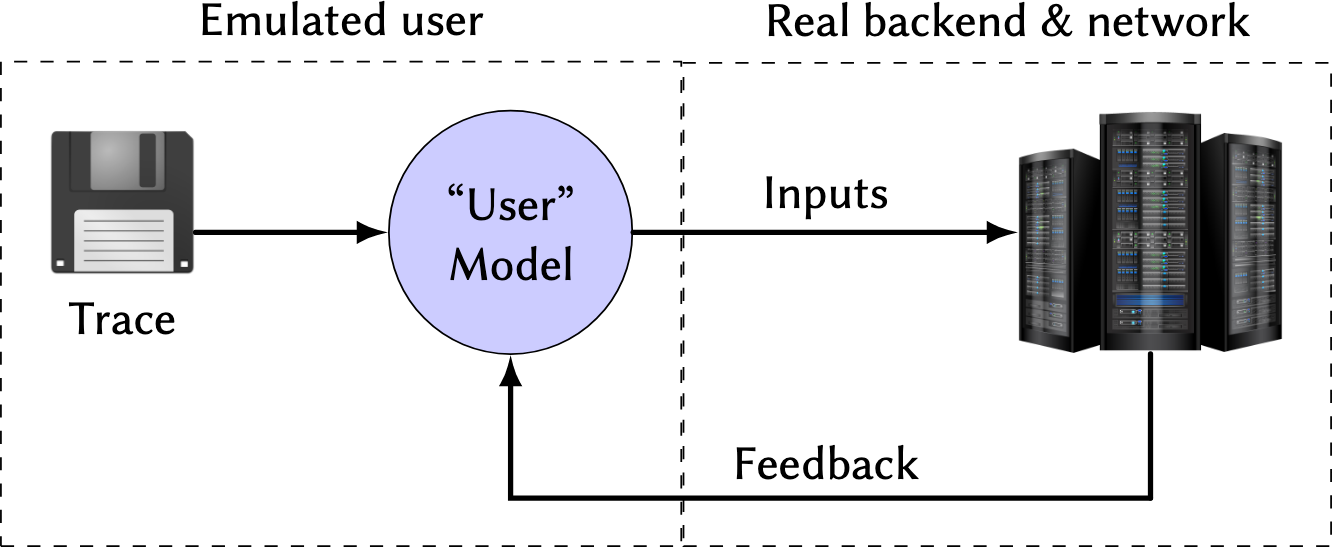
\includegraphics[width=\textwidth]{Figs/trace_edgedroid.png}
        \caption{%
            High level conceptual design of our methodology for \gls{WCA}.
            We replace the human by a trace-driven emulation.
            This allows us to maintain realism in inputs sent over the network to the compute process on the backend, while simplifying the design of the client software.
        }
    \end{subfigure}
    \hfill
    \begin{subfigure}[b]{.47\textwidth}
        \centering
        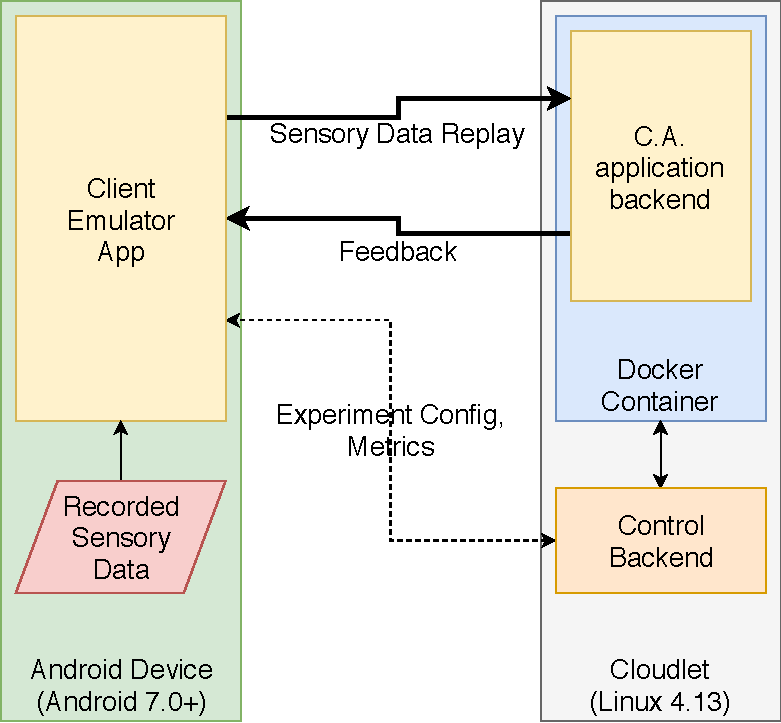
\includegraphics[width=\textwidth]{publications/2018DemoScalingOnTheEdge/img/TraceReplay_GenArch}
        \caption{%
            Architectural overview of the EdgeDroid \num{1.0} tool.
            The ``client emulator app'' implements the aforementioned user model together with the required networking functionality to connect to a \gls{WCA} backend running on a cloudlet.%
        }
    \end{subfigure}\\
    \medskip
    \begin{subfigure}[t]{\textwidth}
        \centering
        \adjustbox{scale=0.7}{
            \begin{tikzpicture}[align=center,
                node distance=.5cm and 1.5cm,
                every initial by arrow/.style={-{Latex[length=2mm]}}]
                % Place nodes
                \node [initial, state, minimum size=6em, initial text=] (play) {Play};
                \node [state, above right=of play, minimum size=6em] (change) {Change\\step};
                \node [state, below right=of play, minimum size=6em] (rewind) {Rewind};
                \node [state, accepting, above right=of rewind, minimum size=6em] (shutdown) {Shutdown};

                % Draw edges
                \path[draw, -{Latex[length=2mm]}]
                (play) edge [bend right=20] node[left] {Step done} (rewind)
                edge [bend left=20] node[left] {Got feedback\\(\emph{positive})} (change)
                edge [out=140,in=220,looseness=6] node[left] {Step\\not done} (play)

                (change) edge [bend left=20] node[right] {Step changed} (play)
                edge [bend left=20] node[right] {All steps done} (shutdown)

                (rewind) edge [bend right=20] node[right] {Rewound} (play)
                edge [bend right=20] node[right] {Too many rewinds} (shutdown);

            \end{tikzpicture}
        }
        \caption{State diagram of the user model governing the replay of the pre-recorded trace at runtime. This model approximates the behavior of an ``ideal'' human, one that is patient and makes no mistakes.}\label{fig:usermodel}
    \end{subfigure}
    \caption{%
        Overview of our first implementation of the methodology for \gls{WCA}.
    }\label{fig:edgedroid1:trace}
\end{figure}

We first introduce our methodology in \cref{paper:olguinmunoz2018demoscaling,paper:olguinmunoz2019edgedroid}.
The former corresponds to an extended abstract paper which discusses a high level overview of our approach; the latter presents a deeper, more complete discussion about the implementation together with some first experimental results.

The overall goal of these papers is to explore this methodological approach as applied to \gls{WCA}.
As discussed in \cref{chap:introduction}, the main challenge to benchmarking \gls{WCA} --- and other ``human-in-the-loop'' applications on the edge --- concerns the involvement of human beings in their operation.
Humans are unreliable, and, perhaps more importantly, hard to scale.
\todo[inline]{More reasons}

The implementation of the client-side emulation necessary for our methodology follows in these works a trace-based design.
We introduce a tool, \emph{EdgeDroid \num{1.0}}, which replays a pre-recorded trace of sensory inputs to the original \gls{WCA} backend.
The tool is implemented in Android, allowing for its easy deployment on the same kind of \gls{COTS} mobile devices on which real \gls{WCA} applications are intended to run in the future.
Furthermore, this tool is instrumented, allowing us to collected a multitude of system-level metrics at runtime which can then be analyzed.
On the other hand, the trace in question corresponds to a pre-recorded sequence of sensory inputs obtained from a real execution of the \gls{WCA} by a human volunteer.
The trace is recorded in a near-ideal setting, such that it does not include either human mistakes or segments with degraded system responsiveness.
Once recorded, the trace is manually segmented into the logical component steps of the task, and these are replayed in sequence back to the backend by the EdgeDroid tool.

We opt for a trace-based approach for our first implementation of the methodology for \gls{WCA} for three key reasons.
The first of these is the level of realism if affords in terms of the payloads sent over the network and, in particular, processed by the backend.
Using a trace ensures that the same computation is performed on the edge as if a human was involved, while also ensuring a reproducible application execution path.

The second is simplicity, as such an approach does not require complex modeling of human behavioral patterns, merely the observation and recording of them.
Compatible traces can be easily obtained simply by instrumenting existing \gls{WCA} client applications to record all captured inputs.

The final advantage corresponds to extensibility.
As long as the tasks belong to the same category of \gls{WCA} applications (in this case, step-based cognitive assistance), using a trace makes extending the tool to different tasks merely a matter of recording a new trace.

\todo[inline]{}

\subsection{Applying the methodology to \acsp{NCS}}

\todo[inline]{}

\subsection{Construction of a testbed for the implementation of the methodology}\label{sec:testbed}

\todo[inline]{}
